\section{Experiments and Results }  \label{section:experimentresults}


\subsection{Experiments}

Our approach is composed of 4 main stages. Such as - (1) 2D matching between try-on cloth image and SMPL\cite{Loper2015SMPLAS} model silhouette, 



\subsection{Results}



\begin{figure*}[t]
   \centering
\begin{tabular}{cc|cc|cc}

Try-on cloth&Target human&GMM\cite{Wang2018TowardCI})&TOM\cite{Wang2018TowardCI})&Warped(Ours)&Try-on(Ours)\\

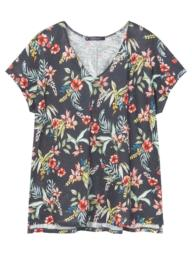
\includegraphics[width=2cm]{figures/cloth/002353_1.jpg}&
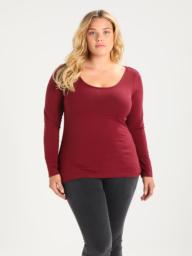
\includegraphics[width=2cm]{figures/image/007029_0.jpg}&
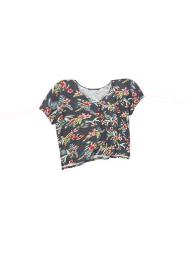
\includegraphics[width=2cm]{figures/cp-vton/warp-cloth/002353_1_007029_0.jpg}&
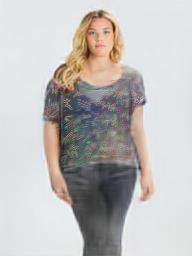
\includegraphics[width=2cm]{figures/cp-vton/try-on/002353_1_007029_0.jpg}&
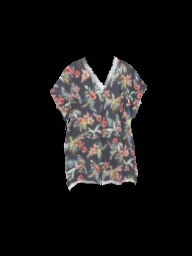
\includegraphics[width=2cm]{figures/c3dwfull/002353_1_007029_0.png}&
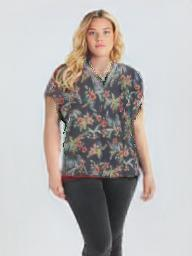
\includegraphics[width=2cm]{figures/try-on/002353_1_007029_0.jpg}\\

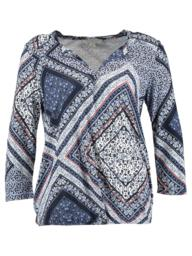
\includegraphics[width=2cm]{figures/cloth/016962_1.jpg}&
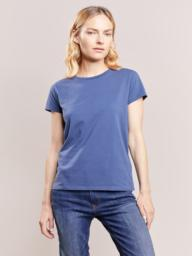
\includegraphics[width=2cm]{figures/image/005379_0.jpg}&
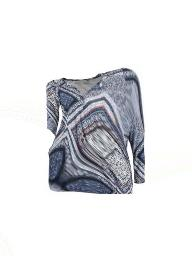
\includegraphics[width=2cm]{figures/cp-vton/warp-cloth/016962_1_005379_0.jpg}&
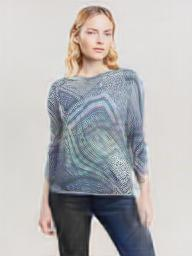
\includegraphics[width=2cm]{figures/cp-vton/try-on/016962_1_005379_0.jpg}&
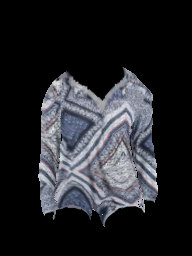
\includegraphics[width=2cm]{figures/c3dwfull/016962_1_005379_0.png}&
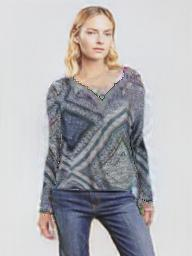
\includegraphics[width=2cm]{figures/try-on/016962_1_005379_0.jpg}\\

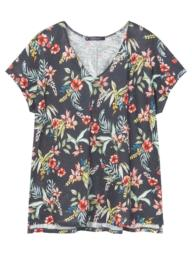
\includegraphics[width=2cm]{figures/cloth/002353_1.jpg}&
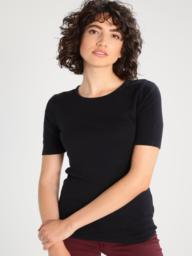
\includegraphics[width=2cm]{figures/image/019581_0.jpg}&
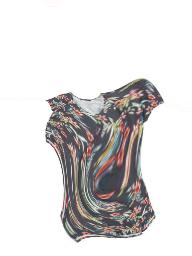
\includegraphics[width=2cm]{figures/cp-vton/warp-cloth/002353_1_019581_0.jpg}&
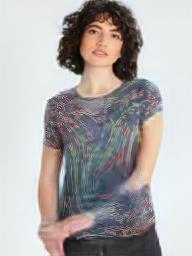
\includegraphics[width=2cm]{figures/cp-vton/try-on/002353_1_019581_0.jpg}&
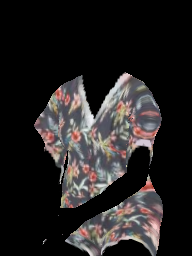
\includegraphics[width=2cm]{figures/c3dwfull/002353_1_019581_0.png}&
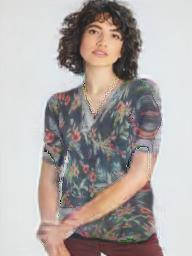
\includegraphics[width=2cm]{figures/try-on/002353_1_019581_0.jpg}\\

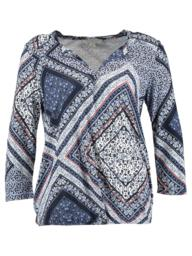
\includegraphics[width=2cm]{figures/cloth/016962_1.jpg}&
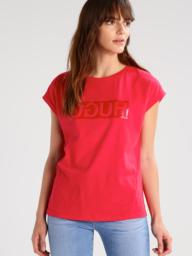
\includegraphics[width=2cm]{figures/image/019402_0.jpg}&
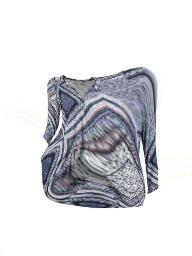
\includegraphics[width=2cm]{figures/cp-vton/warp-cloth/016962_1_019402_0.jpg}&
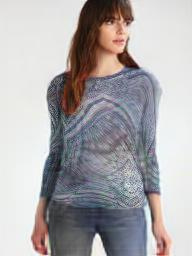
\includegraphics[width=2cm]{figures/cp-vton/try-on/016962_1_019402_0.jpg}&
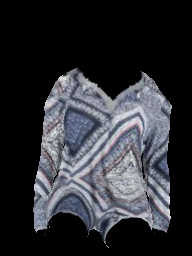
\includegraphics[width=2cm]{figures/c3dwfull/016962_1_019402_0.png}&
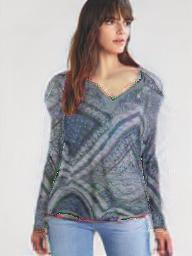
\includegraphics[width=2cm]{figures/try-on/016962_1_019402_0.jpg}\\

\end{tabular}

    \caption{Qualitative comparison between the baseline CP-VTON\cite{Wang2018TowardCI} and our approach. For each row, first pair of images are the inputs, try-on cloth and target human. Second pair is the warped cloth and final try-on results of CP-VTON\cite{Wang2018TowardCI}. And last pair includes the results of our approach; 3D reconstructed-deformed cloth, and the try-on results from the blending network.}
    \label{fig:testresults}
\end{figure*}



Figure \ref{fig:testresults} shows qualitative comparison results between the state-of-the-art image-based virtual try-on model CP-VTON\cite{Wang2018TowardCI} and our approach.



\subsection{Failure cases}

Although, our approach can reconstruct fashion clothes while preserving the clothing characteristics e.g. texture, color, shape realistically, there are cases where it fails to transfer cloth model to the target human and later in try-on. Especially the cases where SMPLify\cite{Bogo2016SMPLify} optimizations are mismatched. Additionally, as mentioned in Section \ref{section:tryon}, due to differences in training data and testing data of try-on/blending network, final try-on outputs gets worse.



\begin{figure*}[t]
   \centering
\begin{tabular}{cccc}

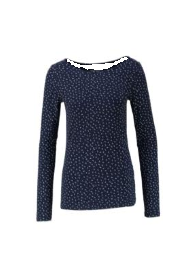
\includegraphics[width=1cm]{figures/c2dw/000118_1.png}&
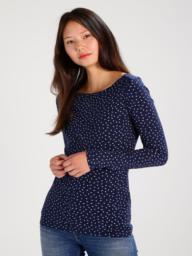
\includegraphics[width=1cm]{figures/image/000118_0.jpg}&
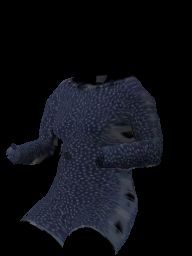
\includegraphics[width=1cm]{figures/c3dwfull/000118_1_000118_0.png}&
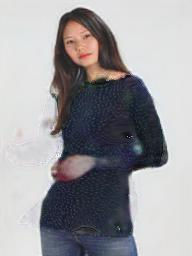
\includegraphics[width=1cm]{figures/try-on/000118_1_000118_0.jpg}\\

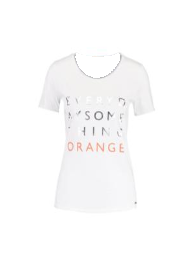
\includegraphics[width=1cm]{figures/c2dw/004508_1.png}&
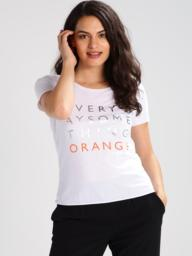
\includegraphics[width=1cm]{figures/image/004508_0.jpg}&
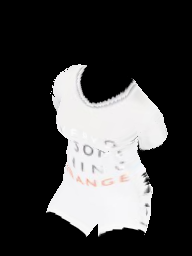
\includegraphics[width=1cm]{figures/c3dwfull/004508_1_004508_0.png}&
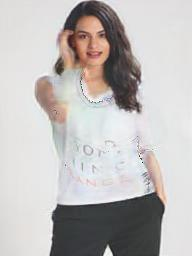
\includegraphics[width=1cm]{figures/try-on/004508_1_004508_0.jpg}\\

Cloth(2D)&Target&Cloth(Warped)&Try-on\\

\end{tabular}

    \caption{Failure cases}
    \label{fig:clothtransfertryon}
    
\end{figure*}



